

\section{Backend}

\begin{figure}[h]
\centerline{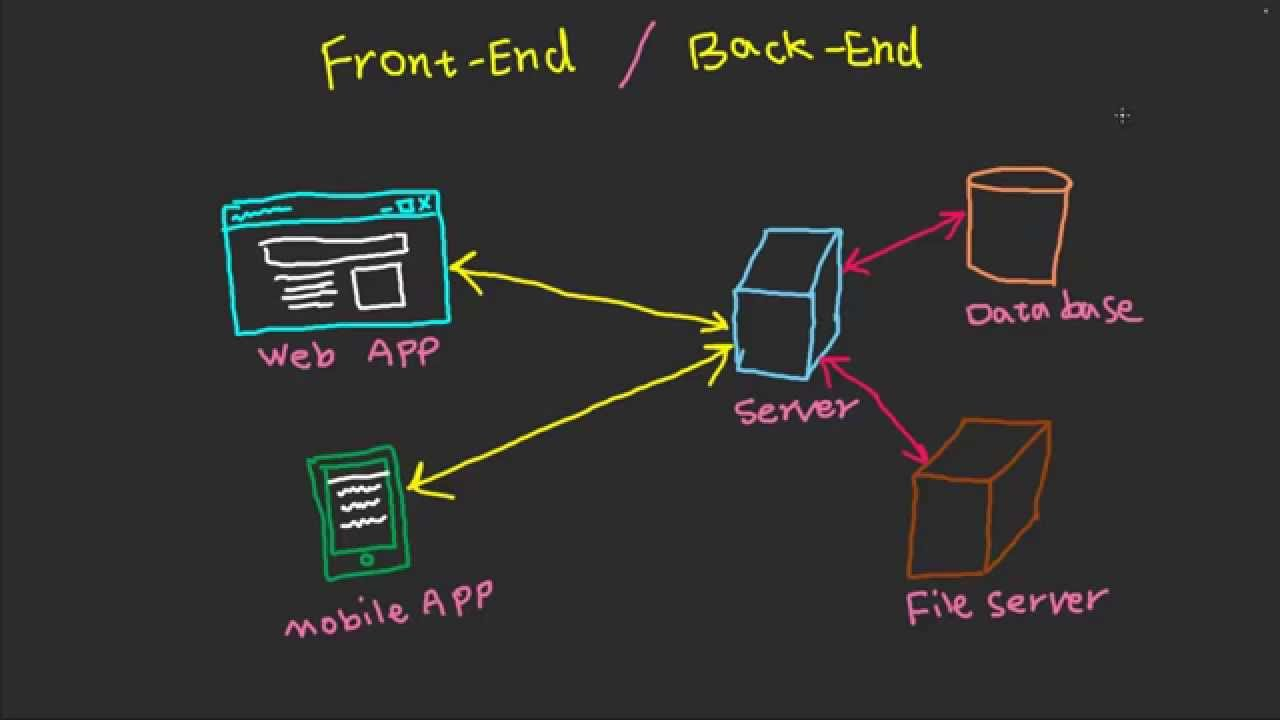
\includegraphics[width=1\textwidth]{figures/backend.jpg}}
\caption{Backend}
\end{figure}

Back-end atau server-side adalah merupakan bagaimana sebuah website berkerja, meng-update
dan berubah. back-end adalah sesuatu system yang dimana User tidak akan dapat melihatnya di dalam browser,
seperti Database dan Server. biasanya orang - orang yang bekerja di bagian back-end di panggil atau disebut sebagai
Programmers atau Developer. Back-end developers adalah orang yang paling khawatir tentang hal - hal yang menyangkut keamanan,
struktur sistem dan manajemen konten. sebenarnya para back-end develper juga mengetahui tentang front-end seperti HTML dan CSS.
namun itu bukanlah bidang mereka bekerja. 

\subsection{Backend System}
Pada system dan metode  yang membuat informasi dapat digunakan secara oromatis untuk mengakses pada fungsionalitas system computer backend yang digunakan ke server aplikasi. Metode inivjuga dapat beroperasiuntuk menghubungkan ke system computer backend dan memperoleh fungsionalitas untuk menentukan informasi  pada system backend. Dan pada informasi yang diperoleh dan dapat dianalisis secara terprogram,dan informasi yang sangat baru dapat dianalisis yang dimana informasi dibuat secara terprogram dapat digunakan untuk mengakses fungsionalitas system backend.

Back-end biasanya mengacu pada program dan skrip yang bekerja di dalam server, untuk membuat sebuah halaman web yang dinamis dan interatif. Back-end memiliki tugas-tugas yaitu seperti :

Desain Informasi pada web
Pemrosesan form
Pemrograman dalam database
Aplikasi Berbasis Web

Dari tugas - tugas tersebut Back-end memiliki tiga bagian diantaranya yaitu server,aplikasi, dan database.

\section{Bahasa Pemrograman yang digunakan di Backend}

\begin{figure}[h]
\centerline{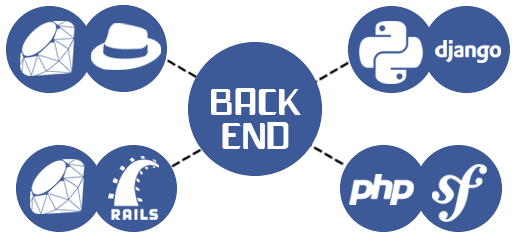
\includegraphics[width=1\textwidth]{figures/bahasa.png}}
\caption{Bahasa Pemrograman yang dipakai di Backend}
\end{figure}


\subsection{C}
Bahasa Pemrograman Backend yang biasa digunakan developer ialah C, C++, dan Java .
Bahasa C adalah suatu perkembangan dari bahasa B yang di kembangkan oleh Ken Thompson pada tahun 1980.
Bahasa C rilis pertama kali ditulis oleh Brian W. Bahasa C, awalnya digunakan oleh sistem operasi UNIX.
Bahasa C adalah bahasa pemrograman tingkat standar, bahasa C memiliki kegunaan yang sering di gunakan
diantaranya untuk membuat perangkat lunak.

\subsection {C++}

Pengertian C++ adalah “multi-paradigm,” artinya anda dapat menulis suatu kode, caranya procedural tapi juga bisa menggunakan fungsional,berorientasi objek, dan campuran paradigm suatu pemrograman.  Bahasa pemrograman C++ ini bisa lebih sulit untuk dipelajari; kita dapat mengembangkan dengan menggunakan satu atau lebih dari model ini,  atau kita dapat menggabungkan dengan Bahasa pemrograman lainnya.

 \subsection {C\#}
Sedangkan C\# merupakan sebuah bahasa programming yang simple, modern, OOP dan aman untuk penggabungannya dengan beberapa bahasa programming lain.


\subsection {PHP}
 	adalah salah satu server side untuk dirancang khusus untuk aplikasi web dan PHP disisipkan diantara bahasa HTML sebab bahasa server side, maka dieksekusi diserver. sehingga yang kirimkan ke browser adalah hasil jadi dalam bentuk HTML. PHP termasuk Open Source Product dapat diubah disource code dan mendistribusikan secara bebas.

\subsection{Python}
Python merupakan  bahasa pemrograman yang serba guna atau bersifat open source. Python lebih menekankan pada pembacaan  kode agar lebih mudah untuk memahami sintaks. Hal tersebut membuat bahasa pemrograman python lebih mudah dipelajari baik pemula maupun untuk yang sudah menguasai bahasa pemrograman ini dan dilengkapi dengan fungsionalitas standar besar serta komprehensif. Pyhton telah digunakan untuk mengembangkan berbagai macam perangakat lunak, seperti internet scipting, system programming, user interfaces, prudect customization, numberic programming. Pada saat ini bahasa pemrograman pyhton menduduki posisi 4 atau 5 paling sering digunakan diseluruh dunia.

\subsection{Perl}
Proxy server ialah suatu komputer atau beberapa komputer yang diletakkan sebagai pelayanan kepada pelanggan yang ingin mengajukan layanan data baik dari pusat komputer(server).
Proxy server sering disebut sebagai media cache terhadap suatu konten website. Di ruang lingkup pendidikan pada laboratorium komputer jaringan di Institusi Sains \& Teknologi ditemukan jaringan yang belum ada penanganan masalah internet yang diakses berkali-kali sehingga bandwidth pada internet tidak efektif, penelitian ini bertujuan  untuk melakukan suatu penyimpanan konten yang diakses ke dalam proxy server kemudian melakukan filter konten menggunakan pemrograman PERL.
Ini dilakukan melalui proxy server, yaitu melalui fungsi pada cachig dan filter pada proxy server dengan menggunakan pemrograman PERL dan regex pada PERL.

\subsection{ASP .NET}
ASP.NET merupakan produk dari teknologi Microsoft untuk pengembangan aplikasi berbasis web dinamis. 
Bahasa pemrograman ini mempermudah pada pemula maupun yang sudah menguasai bahasa pemrograman ini , dikarenakan memberikan solusi pada pengembang untuk mendesign aplikasi web dengan cepat, mudah dan efisien. 
ASP diproses melalui web server dan menghasilkan HTML untuk dikirimkan pada web browser.



\subsection{Java}
Dalam backend juga menggunaka javascript yaitu suatu format teks untuk mengserialisasi data yang terstruktur yang berasal dari objek literal JavaScripts.Pada JavaScript dapat mewakili dari empat tipe yaitu string, angka, boolean, dan nul, dan ada juga dua tipe terstruktur yaitu objek dan array. Objek kumpulan yang tanpa batas dari nol ata lebih dari nama atau nilai pasangannya, yang dimana nama ialah string sedangkan nilai ialah angka, boolean, objek, dan null. Array yaitu urutan dari nol atau melebihi banyak nilai.

\subsection{Ruby}
Ruby merupakan bahasa pemrograman yang stabil, dengan menggabungkan bahasa pemrograman favoritnya seperti Perl, smalltalk, Eiffel, dan Lisp.
Membentuk suatu bahasa pemrograman baru yang menyeimbangkan pemrograman fungsional dengan imperatif.
Bahasa pemrograman Ruby mempunyai sistem yang dengan otomatis akan langsung terhapus semua data-data yang tidak terpakai dan tidak digunakan lagi pada memori. 
Platform sistem operasi yang mendukung bahasa pemrograman Ruby yaitu sistem operasi Linux, Unix, Amiga, Symbian, Mac dan Windows.

\section{Database Backend}
Pada sistem basis data yaitu telah lama dilanda masalah kinerja pada penigkatan dalam penggunaan mainframe atau di dalam aplikasi basis data. Dan solusi untuk masalah ini yaitu dengar membongkar sistem basis data dari komputer mainframe ke komputer backend. Pada komputer itu memiliki penyimpanan disk sendiri, digunakan juga untuk melakukan semuoa operasi data base, dan saling berinteraksi dengan mainframe.


\section{Arsitektur Three-Tier}
Didalam masalah arsitektur two-tier telah diupdate ke tingkat tertentu dengan memperluas dari dua tingkat menjadi tiga tingkat.
Arshitektur three-tier akan mengisolisasi pemrosesan data dari lokasi pusat yang dapat dengan mudah diubah tanpa melibatkan dan mepengaruhi klien. Di dalam arsitektur three-tier ini, logika presentasi berada pada tingkat pertama (klien), logika bisnis berada pada 
tingkat menengah, dan yang lainnya seperti database berada di tingkatan ketiga yaitu back-end. Di tingkat menengah dalam
arsitektur three -tier (server aplikasi) akan menangani pemrosesan data dan akan menjadi antarmuka antara front - end (klien) dan
tingkat back-end (database).


\section{Web Service}
Web Service merupakan penyatuan dari 2 aspek yaitu Web dan Service, yang mana penjelasan Web dan Service akan dijelaskan di bawah ini :

\subsection{WEB}
pertama - tama disini akan dijelaskan tentang Web, Web merupakan website yang berarti jaringan yang dapat mengakses situs

\subsection{Service}
Service merupakan layanan, yang dimana digunakan untuk melayani dan melakukan pelayanan

sehingga dari kedua perihal diatas dapat disimpulkan bahwasanya web service adalah sebuah jaringan global yang memiliki pelayanan atau keamanan,
didalam web service user diberikan layanan berupa keamanan dalam berselancar di Internet. macam - macam model dari web service adalah sebgai berikut ini :

\begin{enumerate}
\item SOAP (Simple Object Access Protocol)
\item WDSL (Web Service Description Language)
\item RDF (Resource Description Framework)
\item RSS (Really Simple Syndication)
\end {enumerate}


\section{Backend Developer}
Orang yang bekerja di bagian back-end atau bisa kita sebut seorang back-end developer adalah seorang programmer yang hanya
memusatkan atau berfokus pada bagian keamanan, desain sistem, dan management data pada sistem. Seorang back-end developer
sangat dibutuhkan dalam melakukan pengembangan sistem atau sebuah aplikasi yang dinamis atau aplikasi yang memiliki data selalu
berubah - ubah, contohnya website yang dinamis seperti facebook dan google.

\section{Backend as a Service}
Baas adalah sebuah provider untuk web dan mobile app developer untuk dapat mengkoneksikan 
aplikasi mereka ke dalam system penyimpanan cloud backend sekaligus masih tetap melakukan proses yang lain seperti user management, 
mendapatkan notifikasi, bermain social media, dan fitur – fitur lainnya yang terdapat di dalam aplikasi mobile mereka saat ini.

\subsection{Kelebihan yang dimiliki BaaS}
Tujuan dari BaaS adalah untuk membuat hidup developer menjadi 
lebih mudah. BaaS ada karena kurangnya keahlian dari seorang 
mobile developer dan tingginya tingkat permintaan user untuk 
aplikasi smartphone mereka. berikut ini adalah kelebihannya :

\begin{enumerate}
\item Keuntungan yang efisien
\item Lebih cepat waktu penjualannya
\item Aplikasi didelivery dengan sumber daya yang lebih sedikit
\item Ter-optimisasi untuk mobile dan tablet
\item Aman dan terukur
\item Penggunaan sumber daya API yang umum dipakai
\end{enumerate}

\subsection {Yang dapat anda buat dengan menggunakan BaaS}
\begin{enumerate}
\item Pengembangan Website
\item Mobile Aplikasi, dll
\end{enumerate}

\section{JSON (JavaScript Object Notation)}
	merupakan sebuah format pertukaran data yang mudah dibaca atau dimengerti dan dituliskan oleh manusia, 
serta JSON memiliki kemudahan untuk diterjemahkan dan juga diubah \(generate\) oleh sebuah mesin \(Computer\).
JSON adalah sebuah format teks yang tidak memiliki ketergantugan pada Bahasa pemrograman manapun karena JSON menggunakan 
gaya penulisannya sendiri yang mana dia menggunakan Bahasa – Bahasa pemrograman yang sudah umum seperti C family, Java, 
JavaScript, Perl, Python dan lainya, dan menjadikannya sebagai sebuah format yang tetap miliknya sendiri.
hal tersebutlah yang menjadikan JSON sebagai format pertukaran data yang ideal didalam dunia pemrograman. 


\section{Mobile Backend Starter}
Backend tidak hanya dipakai oleh web yang dinamis namun akhir - akhir ini google telah menambahkan sebuah layanan yang bernama
"Mobile Backend Starter", google menambahkan layanan tersebut dengan tujuan untuk memudahkan pengguna untuk menggunakan
layanan awan berupa "Cloud Services" dalam sebuah aplikasi mobile yang akan dikembangkan. Ketersediaan dari layanan "Mobile Backend Starter" ini bebas digunakan untuk publik.



		

